\documentclass[main.tex]{subfiles}

\begin{document}

  \section{Superelliptic curves}\label{sec:se_curves}

  \subsection{Definition \& properties}
    
    \begin{defn}\label{def:se_curve}
%        A superelliptic curve over a field $K$ is a smooth cyclic branched covering of the projective line 
%        $\cu \rightarrow \P^1_K$ of degree $m > 1$ such that $\text{char}(K)$ and $m$ are coprime.
    In this paper, a superelliptic curve $\cu$ over $\C$ is a smooth plane projective curve that has an affine model given by an equation of the form 
   \begin{align}\label{eq:aff_model}
    \caff : \quad y^m = f(x) \;= \; c_f \cdot \prod_{k=1}^d (x-x_k)\,,
   \end{align}
   \end{defn}
   where $m > 1$ and $f \in \C[x]$ is separable of degree $d \ge 3$. 
   Without loss of generality we may assume $c_f = 1$ (if not, apply the transformation $(x,y) \mapsto (x,\sqrt[m]{c_f}\,y)$\,).  \abstand
   Over $\C$ we identify the curve $\cu$ with the Riemann surface $\cu(\hat{\C})$ and denote by $\pr : \cu \rightarrow \P^1_{\C}$ the corresponding smooth cyclic branched covering of the projective line
   defined by the $x$-coordinate.
   
  There are $\delta = \gcd(m,d)$ points above infinity $P_{\infty}^{(1)},\dots,P_{\infty}^{(\delta)} \in \cu$, that behave differently depending on $m$ and $d$ (see \cite{CT1996}, \S 1 for details). 
  Especially, $\infty \in \P^1_{\C}$ is a branch point for $\delta \ne m$. Thus, we introduce the set of finite branch points $X = \X$ as well as the set of all branch points
  \vspace{-0.3cm}
  \begin{align}\label{eq:branch_points}
         \hat{X} = \begin{cases}   X \cup \{ \infty \}, \quad \text{if} \; m \, \nmid \, d\,,\\
         X,\quad \text{otherwise.}
     \end{cases}
  \end{align} 
  As we will see in \S \ref{subsec:roots_branches} the ramification indices at the branch points are given by $e_x = m$ for all $x \in X$ and $e_{\infty} = \frac{m}{\delta}$\,. Using the
  Riemann-Hurwitz formula, we obtain the genus of $\cu$ as
   \vspace{-0.3cm}
  \begin{align}\label{eq:genus}
    g = \frac{1}{2}( (d-1)(m-1) - \delta + 1)\,.
  \end{align}

   

  
  \subsection{Complex roots and branches of the curve}\label{subsec:roots_branches}

  \subsubsection{The complex mth root}

  Working over the complex we encounter several multi-valued functions
  which we will briefly discuss here.  Closely related to superelliptic
  curves over $\C$ is the complex $m$-th root.
  Before specifying a branch it is a multi-valued function $y^m = x$
  that defines an $m$-sheeted Riemann surface, whose only branch points
  are at $z = 0,\infty$, and they're totally ramified.

  For $z\in\C$, it is natural and computationally convenient to use the
  principal branch of the $m$-th root
  \begin{equation}
      \sqrt[m]z \text{ such that } -\frac{π}m<\arg(\sqrt[m]z)\leq\frac{π}m
  \end{equation}
  which has a branch cut along the negative real axis $]\!-\infty,0[$.
  Crossing it in positive orientation corresponds to multiplication by
  the primitive $m$-th root of unity
  \begin{equation}
  \zeta = \zeta_m = e^{\frac{2\pi i }{m}}    
  \end{equation}
  on the surface. In
  particular the monodromy at $z=0$ is cyclic of order $m$.

  \subsubsection{Superelliptic curves}

  Now the superelliptic curve $\cu:y^m=f(x)$ is also a Riemann surface with
  $m$ sheets.
  We call \emph{branch of $\cu$} a function $y(x)$ such that
  $y(x)^m = f(x)$ for all $x \in \C$. At every $x$, the branches of $\cu$ only
  differ by multiplication by a power of $\zeta$.
  

  In the case of superelliptic curves given
  by an affine model $\caff : y^m = \prod_{k = 1}^d (x - x_k)$, indepently of
  $d$ and $m$, every finite branch point $x_k$ is totally ramified, which means
  the local monodromy is given by a cyclic permutation $\sigma_k \in S_m$.
  
  As we shall see below, we
  will not impose a global ordering on the sheets of $\cu$. Instead we use
  locally analytic branches $\yab$ (see \ref{def:yab}) and order them such that
  moving one sheet up corresponds to the transformation $\yab \mapsto
  \zeta\yab$. For us, encircling a branch point in positive orientation means
  applying the local monodromy to the analytic branches of $\cu$, therefore we
  can therefore assume that $\sigma_k = \sigma$ for $k = 1,\dots,d$.
 
  \subsubsection{Local branches}
  
  In order to integrate holomorphic forms on $\cu$
  it is crucial to be able to follow an explicit analytic continuation of $y$ along a
  path joining two branch points $a$ and $b$.
  
  One could of course consider the principal branch of the curve
  \begin{equation}
      y(x) = \sqrt[m]{f(x)}
  \end{equation}
  however this is not a good model to compute with: it has branch cuts
  wandering around the $x$-plane.

  Instead, let us first consider the affine transformation
  \begin{equation}
      \label{def:uab}
      u_{a,b} : x \mapsto \frac{b-a}{2}\left(x+\frac{b+a}{b-a}\right) 
  \end{equation}
  which depends on two branch points $a,b$ and maps $[a,b]$ to $[-1,1]$.

  Then we define the local branch
  \begin{equation}
      \label{def:yab}
      \yab(x) =   C_{a,b} \sqrt[m]{1 - u_{a,b}(x)^2}
      \prod_{x_k\neq a,b}\sqrt[m]{u_{a,b}(x)-u_{a,b}(x_k)}
  \end{equation}
  where
  \begin{equation}
      C_{a,b} = \left(\frac{b-a}{2}\right)^{\frac{d}{m}} e^{\frac{\pi i}{m}}
  \end{equation}
  is chosen so that $y_{a,b}^m = f(x)$.

  This is a branch of $\cu$, whose branch cuts are all parallel to $(a,b)$,
  which is holomorphic inside $]a,b[$ and has two outward cuts $]\infty, a]$ and $[b,\infty[$.

  In fact it is convenient to work with the local $u$ variable: let $u_k = u_{a,b}(x_k)$ be the image
  of all branch points, then the function
  \begin{equation}
      \ft_{a,b}(u) = \prod_{x_k \ne a,b} \sqrt[m]{u - u_k}
  \end{equation}
  is holomorphic on a neighborhood $U_{a,b}$ of $[-1,1]$ which we can take as
  any ellipse\footnote{we will exhibit such a neighborhood in section \ref{sec:gc_ellipse}}
  containing no $u_k\neq\pm1$ , while
  \begin{equation}
      \sqrt[m]{1-u^2}
  \end{equation}
  has two cuts $]-\infty,-1]$ and $[1,\infty[$, and is holomorphic on the complementary
  $\overline U$ of these cuts.

  \begin{figure}[H] \begin{center} % Tikz File 'tikz_pic_14.tex'
% \documentclass{standalone}
% \usepackage{tikz}
% \usetikzlibrary{arrows}
% \usetikzlibrary{shapes.misc}
% \usetikzlibrary{decorations.markings}
% \tikzset{cross/.style={cross out, draw=black, minimum size=2*(#1-\pgflinewidth), inner sep=0pt, outer sep=0pt},cross/.default={1pt}}
% \tikzset{
%     halfarrow1/.style={postaction={decorate},
%         decoration={markings,mark=at position .5 with
%         {\arrow[line width=0.4mm]{>}}}} }
% \tikzset{
%     halfarrow2/.style={postaction={decorate},
%         decoration={markings,mark=at position .5 with
%         {\arrow[line width=0.4mm]{<}}}} }
% \begin{document}
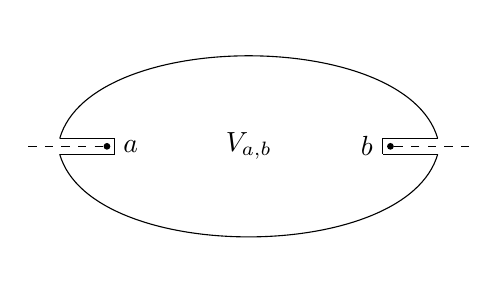
\begin{tikzpicture}

  \draw (-1.5,0) node {$a$};  \draw (1.5,0) node {$b$}; \draw (0,0) node {$V_{a,b}$};
  \filldraw [black] (-1.8,0) circle (1pt); \filldraw [black] (1.8,0) circle (1pt);
    \draw [dashed] (-2.8,0) -- (-1.8,0);   \draw [dashed] (2.8,0) -- (1.8,0);
    \draw (-2.4,0.1) .. controls (-2,1.5) and (2,1.5) .. (2.4,0.1);
    \draw (-2.4,-0.1) .. controls (-2,-1.5) and (2,-1.5) .. (2.4,-0.1);
    \draw (-2.4,-0.1) -- (-1.7,-0.1); \draw (2.4,-0.1) -- (1.7,-0.1);
    \draw (-2.4,0.1) -- (-1.7,0.1); \draw (2.4,0.1) -- (1.7,0.1);
    \draw (-1.7,0.1) -- (-1.7,-0.1); \draw (1.7,0.1) -- (1.7,-0.1);

\end{tikzpicture}


  \end{center} \caption{Area of holomorphicity for $\yab$\,.}
  \label{fig:set_vab} \end{figure}

  We call $V_{a,b} = u_{a,b}^{-1}(U_{a,b}\cap \overline U)$ the inverse image of their intersection,
  so that $V_{a,b}$ is an ellipse shaped neighborhood of $]a,b[$ with two segments removed
      (see Figure \ref{m-fig:set_vab})
      on which the local branch $\yab$ is well defined and holomorphic.

  With these notations, we now have
  \begin{prop}
     \begin{itemize}
         \item $\ft_{a,b}$ is holomorphic and does not vanish on $U_{a,b}$
         \item $y_{a,b}(x) = C_{a,b} \ft_{a,b}(u(x)) \sqrt[m]{1-u(x)^2}$ is holomorphic
         on $V_{a,b}$
         \item $y_{a,b}^m = f(x)$ for all $x\in\C$
     \end{itemize} 
     Moreover, we can assume that moving up $l$ sheets on $\cu$
     corresponds to multiplication of $\yab$ by $\zeta^l$. 
 \end{prop}


  \subsection{Cycles and homology}\label{subsec:cycles_homo}
    
   In this paragraph we present an explicit generating set of $\homo$ that is obtained by connecting the locally analytic branches $\yab$\,, as defined in \eqref{def:yab}\,,
   while also taking advantage of the superelliptic structure of our curve.
   For simplicity we will identify all cycles on $\cu$ with their classes in $\homo$\,.
   
   \begin{defn}\label{def:elem_cycle}
   Let $a, b \in X$ be branch points such that $x_k \not\in [a,b]$ for all $x_k \ne a,b$, where  $[a,b]$ is the oriented line segment connecting $a$ and $b$.  
   We define the corresponding \textit{elementary cycle} 
   \begin{align}
    \cyab = \{ \, (x,\yab(x)) \, \mid \, x \in [a,b] \, \} \cup \{ \,(x,\zeta \, \yab(x)) \, \mid \, x \in [b,a] \, \}
   \end{align}
   and, for $l \in \Z/m\Z$, its \textit{shifts}
   \begin{align}
    \cyab^{(l)} = \{ \, (x,\zeta^l \,\yab(x)) \, \mid \, (x,y) \in \cyab \, \}\,. 
   \end{align}
    \end{defn}
    
   By our discussion in \S \ref{subsec:roots_branches}, the $\cyab^{(l)}$ are smooth oriented closed paths in $\pi_1(\cu)$ that are given as concatination of
   lifts of the line segment $[a,b]$ to $\cu$\,. \abstand
   In $\pi_1(\cu)$
   they are homotopic to cycles that encirlce  $a$ in negative and $b$ in positive orientation, once each.
   Assuming the local branch cuts are parallel to $[a,b]$, we have the following useful visualizations of $\cyabl$ on $\cu$.
   \begin{figure}[H]
      \begin{center}
	  % Tikz File 'tikz_pic_13.tex'
\begin{tikzpicture}
     \draw (-1.8,2) node {$a$};  \draw (1.8,2) node {$b$};
     \draw [densely dashed] (-3.0,3) -- (-1.8,3);  \draw [densely dashed] (1.8,3) -- (3.0,3); \draw (-1.8,3) circle (1.3pt); \draw (1.8,3) circle (1.3pt);
      \draw (-1.8,3) -- (1.8,3) [halfarrow2];
   \draw [densely dashed] (-3.0,1) -- (-1.8,1);  \draw [densely dashed] (1.8,1) -- (3.0,1); \draw (-1.8,1) circle (1.3pt); \draw (1.8,1) circle (1.3pt);
\draw (-1.8,1) -- (1.8,1) [halfarrow1];
      
      
      \draw (3.5,2) node {$\sim$};
      
           \draw (5.2,2) node {$a$};  \draw (8.8,2) node {$b$};
     \draw [densely dashed] (4.0,3) -- (5.2,3);  \draw [densely dashed] (8.8,3) -- (10,3); \draw (5.2,3) circle (1.3pt); \draw (8.8,3) circle (1.3pt);
     
\draw (4.5,3) .. controls (4.5,2.4) and (6,2.6) .. (7,3) [halfarrow2];
\draw (7,3) .. controls (8,3.4) and (9.5,3.6) .. (9.5,3) [halfarrow2];

   \draw [densely dashed] (4,1) -- (5.2,1);  \draw [densely dashed] (8.8,1) -- (10,1); \draw (5.2,1) circle (1.3pt); \draw (8.8,1) circle (1.3pt);
\draw (4.5,1) .. controls (4.5,1.6) and (6,1.4) .. (7,1) [halfarrow1];
\draw (7,1) .. controls (8,0.6) and (9.5,0.4) .. (9.5,1) [halfarrow1];
\end{tikzpicture}

      \end{center}
    \caption{Representations of a cycle $\cyabl$.} 
    \label{fig:elem_cycle}
\end{figure}
 
  \bigskip
 
  As it turns out, we do not need all elementary cycles and their shifts to generate $\homo$\,, but only those that correspond to edges in a \emph{maximal spanning tree}, which is constructed
  as follows. \abstand
   Consider the complete graph on the set of finite branch points $G = (X,E')$, i.e.\ $E' = \{ \, (a,b) \, \mid \, a,b \in X \}$\,.
   Each edge $e = (a,b) \in E$ gets assigned a capacity $\tau_e$ that indicates the cost of numerical integration along the interval $[a,b]$\,. \abstand
   Here, the integration process ist most favourable
   between branch points that are far away from the others, that is, according to the double-exponential integration scheme that will be employed. \abstand
   We now apply a standard 'maximal-flow' algorithm from graph theory, based on a greedy approach, that results in a spanning tree $T = (X,E)$, where $E \subset E'$ contains the $d-1$ best edges
   for integration that connect all vertices without producing cycles.
   
   \bigskip
  
  For an edge $e = (a,b) \in E$, we denote by $\gamma_e^{(l)}$ the shifts of the corresponding elementary cycle $\cyab$\,.
  
  \begin{thm}\label{thm:gen_set}
   The cycles $C = \left\{ \, \gamma_{e}^{(l)} \, \mid \, 0 \le l <m-1, \, e \in E \, \right\}$ generate $\homo$.
  \end{thm}
  \begin{proof}
  Denote by $\alpha_a \in \pi(\P^1 \setminus \hat{X})$ a closed path that encircles the branch point $a \in \hat{X}$ exactly once. Then,  due to the relation $1 = \prod_{a \in \hat{X}} \alpha_a$,\,
  $\pi(\P^1 \setminus \hat{X})$ is freely generateted by $\{ \alpha_a \}_{a \in X}$, i.e. in the case $\delta \ne m$ we can omit $\alpha_{\infty}$\,. \abstand
  Since our covering is cyclic, we have that $
  \pi_1(\cu \setminus \pr^{-1}(\hat{X})) = \ker(\pi_1(\P^1 \setminus \hat{X}) \overset{\Phi}{\To} \Aut(\cu \setminus \pr^{-1}(\hat{X})))$. Moreover, $\Aut(\cu \setminus \pr^{-1}(\hat{X})) = C_m 
  \subset S_m$
  and $\Phi(\alpha_a) = (1 \dots m)$ for all $a \in X$. Hence, for every word $\alpha = \alpha_1^{s_1}\dots \alpha_n^{s_n} \in \pi_1(\P^1 \setminus \hat{X})$ we have that
  $\alpha \in \ker(\Phi) \eq \sum_{i=1}^n s_i = 0 \bmod m$. \abstand
  Claim: $\pi_1(\cu \setminus \pr^{-1}(\hat{X})) = \langle \, \alpha_a^{-s} \alpha_b^{s}, \, \alpha_a^m  \, \mid \, s \in \Z, a,b \in X \, \rangle$\,. \\
  Proof: Induction on $n$\,. For $\alpha = \alpha_1^{s_1}$ $m$ divides $s_1$ and therefore $\alpha$ is generated by $\alpha_1^m$. For $n > 1$ we write
  $\alpha = \alpha_1^{s_1}\dots \alpha_n^{s_n} = (\alpha_1^{s_1} \dots \alpha_{n-1}^{s_{n-1}+s_n})(\alpha_{n-1}^{-s_n}\alpha_n^{s_n})$. \abstand
  We obtain the fundamental group of $\cu$ as
  $\pi(\cu) = \pi_1(\cu \setminus \pr^{-1}(\hat{X})) / \langle \, \alpha_a^{e_a} \, \mid \, a \in \hat{X} \, \rangle$, which is generated by 
  $\{ \, \alpha_a^{-s} \alpha_b^{s} \, \mid \, s \in \Z/m\Z, \, a,b \in X \, \}$. (In the case where $\delta \ne 1$, filling in the points above infinity will create additional relations among 
  these generators:
  $1 = (\prod_{a \in X} \alpha_a)^{k \cdot e_{\infty}}$, $k = 1,\dots,\delta-1$\,.) \abstand
  All branch points $a,b \in X$ are connected by a path $(a,v_1,\dots,v_t,b)$ in the spanning tree, so we can write $\alpha_a^{-s} \alpha_b^{s} = (\alpha_a^{-s}\alpha_{v_1}^{s})
  (\alpha_{v_1}^{-s}\alpha_{v_2}^{s})\dots(\alpha_{v_{t-1}}^{-s}\alpha_{v_t}^{s})(\alpha_{v_t}^{-s}\alpha_b^{s})$ and hence we have that 
  $\{ \alpha_a^{-s} \alpha_b^{s} \, \mid \, s \in \Z/m\Z, \, (a,b) \in E \}$ generates $\pi_1(\cu)$ and therefore $\homo$\,. \abstand
%     All that is left to see, is that for each edge $e = (a,b) \in E$ there exists a bijection $\varphi_e$ between
%   $\{ \, \gamma_e^{(l)} \, \mid \, l \in \Z/m\Z \, \} \overset{\varphi_e}{\longleftrightarrow} \{ \, \alpha_a^{-s} \alpha_b^{s} \, \mid \, s \in \Z/m\Z \, \}$\,: \abstand
  If we choose basepoints $p_0 \in P^1 \setminus \hat{X}$ for $\pi_1(P^1 \setminus \hat{X})$ and $P_0 \in \pr^{-1}(p_0)$ for $\pi_1(\cu \setminus \pr^{-1}(\hat{X}))$ and $\pi_1(\cu)$ respectively, then,
  depending on the choice of $P_0$, for all $e = (a,b) \in E$ there exists $l_0 \in \Z/m\Z$ such that $\gamma_e^{(l_0)}$ is homotopic to $\alpha_a^{-1} \alpha_b$ in $\pi_1(\cu,P_0)$. 
   In $\homo$ we have that $\alpha_a^{-s}\alpha_b^{s} = ( \alpha_a^{-1}\alpha_b)^s$, so we obtain the other powers by concatenating
  the shifts $\prod_{l = 0}^{s-1} \gamma_e^{(l_0+l)} = (\alpha_a^{-1}\alpha_b)^s$\,.
  This implies $1 = \prod_{l = 0}^{m-1} \gamma_e^{(l_0+l)} = \prod_{l = 0}^{m-1} \gamma_e^{(l)}$ and 
   $\{ \, \alpha_a^{-s} \alpha_b^{s} \, \mid \, s \in \Z/m\Z \, \} \subset  \langle \, \gamma_e^{(l)} \,
  \mid \, l = 0,\dots,m-1 \,\rangle$ and therefore $\homo = \langle \, C \, \rangle$\,.
  
%   \todo Include $\infty$.\\
%    Each cycle $\alpha \in \homo$ can be encoded as $\alpha = \sum_{k = 1}^d n_kx_k$ with $n_1 + \dots n_d = 0 \bmod m$.
%    Here $n_k \in \Z/m\Z$ indicates that $\alpha$ encircles the branch point $x_k$ $n_k$-times in positive orientation 
%    on neighbouring sheets and the
%    condition on the $n_k$ ensures that $\alpha$ is a closed path.
%    For $e = (a,b)$ we can now write $\gamma_e^{(l)} = a - b$ (Note: $n \cdot \gamma_e^{(l)} = a-b$) , which implies $\sum_{l = 1}^n \gamma_e^{(l-1)} = n(a-b)$, 
%    for $n = 1,\dots,m-1$. \\
%    Since $E$ is a spanning tree, every cycle $x_i - x_j$ involving only two branch points can be written as sum of elements in the spanning tree,
%    i.e. $x_i - x_j = \sum_{e \in E} c_{i,j,e} (x_{e_1}-x_{e_2})$ with $c_{i,j,e} \in \{ \pm 1, 0 \}$. Writing
%    $n_d = -(n_1 + \dots n_{d-1}$) and
%    combining the information, we obtain
%    \begin{align*}
%     \alpha \; & = \; n_1x_1 + \dots n_dx_d = n_1(x_1 - x_d) + \dots + n_{d-1}(x_{d-1} - x_d) \\
%    &  = \;  n_1 \sum_{e \in E} c_{1,d,e} (x_{e_1}-x_{e_2}) + \dots + n_{d-1} \sum_{e \in E} c_{d-1,d,e} (x_{e_1}-x_{e_2}) \\
%    & = \; \sum_{e \in E} c_{1,d,e} n_1 (x_{e_1}-x_{e_2}) + \dots + c_{d-1,d,e} n_{d-1} (x_{e_1}-x_{e_2}) \\
%   &  = \; \sum_{e \in E}  \left( c_{1,d,e} \sum_{l = 1}^{n_1} \gamma_e^{(l)} + \dots +  c_{d-1,d,e} \sum_{l = 1}^{n_{d-1}} 
%   \gamma_e^{(l)} \right) \in \; < C >\,.
% %   & = \sum_{e \in E}  \left( c_{1,d,e} \sum_{l = 1}^{n_1} + \dots + c_{d-1,d,e} \sum_{l = 1}^{n_{d-1}} \right)
% %  \gamma_e^{(l)} 
%    \end{align*}
  \end{proof}

  \begin{rmk}
  \begin{itemize}
   \item[(i)] For $\delta = 1$, we have that $\# C = (d-1)(m-1) = 2g$. Therefore, $C$ is a basis for $\homo$ in that case.
   \item[(ii)] In the case $\delta = m$, the point at infinity is not a branch point. Leaving out one finite branch point in the spanning tree, results in only $d-2$ edges. Hence,
   $\#C = (d-2)(m-1) = 2g$ and $C$ is a basis for $\homo$\,.
  \end{itemize}
  \end{rmk}


  
\subsection{Differential forms}\label{subsec:diff_forms}
  
    The computation of the period matrix and the Abel-Jacobi map requires a basis of $\hd$ as $\C$-vector space. In this section we provide a basis that only 
   depends on $m$ and $d$ and is suitable for double-exponential integration. \abstand
    Among the meromorphic differentials
    \begin{align*}
 \WM = \left\{ \, \omega_{i,j}  \, \right\}_{\substack{1 \le i \le d-1, \\ 1 \le j \le m-1}} \quad \text{with} \quad \omega_{i,j} = \frac{ \dx^i}{i y^j}\,,
  \end{align*}
  there are exactly $g$ that are holomorphic  and they can be found by imposing a simple combinatorial condition on $i$ and $j$.
 

   \bigskip
   
     \begin{prop}\label{prop:holom_diff}
	Let $\delta = \gcd(m,d)$. The following differentials form  a $\C$-basis of $\hd$\,.
	\begin{align}\label{eq:holm_diff}
	  \W =  \left\{ \, \omega_{i,j} \in \WM \, \mid \, -mi + jd - \delta \ge 0 \, \right\}
	\end{align}
     \end{prop}
     \begin{proof}
      First we show that the differentials in $\W$ are holomorphic.
      Let $\w_{i,j} = x^{i-1}y^{-j} \dx \in \WM$. We write down the relevant divisors
      \begin{align*}
       \div(x) & = \sum_{k=1}^m \left(0,\zeta^k{f(0)}^{1/m}\right) - \frac{m}{\delta} \cdot \sum_{l = 1}^{\delta} P_{\infty}^{(l)}\,, \\
       \div(y) & = \sum_{k = 1}^d (x_k,0) - \frac{d}{\delta} \cdot \sum_{l = 1}^{\delta}  P_{\infty}^{(l)}\,, \\
       \div(\dx) & = (m-1)\sum_{k = 1}^d (x_k,0) - \left(\frac{m}{\delta} + 1\right)\cdot \sum_{l = 1}^{\delta}  P_{\infty}^{(l)}\,.
      \end{align*}
     Putting together the information, for $P \in \cu$ lying over $x_0 \in \P^1_{\C}$, we obtain
     \begin{align}\label{eq:diff_cases}
      v_P(\omega_{i,j}) & = (i-1) v_P(x) + v_P(\dx)  - j v_P(y) = 
	\begin{cases}
	 \ge 0\,, \hfill \text{if} \; x_0 \ne x_k,\infty \\
	 = m-1-j \ge 0 \,, \hfill \text{if} \; x_0 = x_k \\
	 = \frac{1}{\delta}(-mi-\delta+jd)\,,\hfill \text{if} \; x_0 = \infty
	\end{cases}\,.
     \end{align}
     We conclude: $\omega_{i,j} \in \WM$ is holomorphic if and only if $\omega_{i,j} \in \W$. \abstand
     Since the differentials in $\W$ are clearly $\C$-linearly independent, it remains to show that
     there are enough of them, i.e. $\#\W = g$. \abstand
     Counting the elements in $\W$ corresponds to counting lattice points $(i,j) \in \Z^2$ in the trapezoid given by the faces
     \begin{align*}
	1 \le i \le d-1\,,\\
	1 \le j \le m-1\,, \\
	i \le \frac{d}{m}j - \frac{\delta}{m}\,.
     \end{align*}
      \begin{figure}[H]
      \begin{center}
	  % Tikz File 'tikz_pic_7.tex'
%\documentclass{standalone}
% \usepackage{tikz}
\usetikzlibrary{arrows}
\usetikzlibrary{shapes.misc}
\usetikzlibrary{decorations.markings}
\tikzset{cross/.style={cross out, draw=black, minimum size=2*(#1-\pgflinewidth), inner sep=0pt, outer sep=0pt},cross/.default={1pt}}
\tikzset{
    halfarrow1/.style={postaction={decorate},
        decoration={markings,mark=at position .5 with
        {\arrow[line width=0.4mm]{>}}}} }
\tikzset{
    halfarrow2/.style={postaction={decorate},
        decoration={markings,mark=at position .5 with
        {\arrow[line width=0.4mm]{<}}}} }
%\begin{document}
\begin{tikzpicture}
%      \draw (-1.8,2) node {$a$};  \draw (1.8,2) node {$b$};
%      \draw (-2.5,3) -- (-1.8,3);  \draw (1.8,3) -- (2.5,3); \filldraw [gray] (-1.8,3) circle (2pt); \filldraw [gray] (1.8,3) circle (2pt);
% \draw (-2.3,3) .. controls (-0.9,2.5) and (-0.9,2.5) .. (0,3) [halfarrow2];
% \draw (0,3) .. controls (0.9,3.5) and (0.9,3.5) .. (2.3,3) [halfarrow2];
% 
%      
%    \draw (-2.5,1) -- (-1.8,1);  \draw (1.8,1) -- (2.5,1); \filldraw [gray] (-1.8,1) circle (2pt); \filldraw [gray] (1.8,1) circle (2pt);
% \draw (-2.3,1) .. controls (-0.9,1.5) and (-0.9,1.5) .. (0,1) [halfarrow1];
% \draw (0,1) .. controls (0.9,0.5) and (0.9,0.5) .. (2.3,1) [halfarrow1];

\draw (-0.7,0) -- (8,0) [->]; \draw (8.5,0) node {$j$};
\draw (0,-0.7) -- (0,4) [->]; \draw (0,4.5) node {$i$};
\draw (1,-0.05) -- (1,0.05); \draw (1,-0.4) node {$1$};
\draw (2,-0.05) -- (2,0.05); \draw (2,-0.4) node {$2$};
\draw (3,-0.05) -- (3,0.05); \draw (3,-0.4) node {$3$};
\draw (4,-0.05) -- (4,0.05); \draw (4,-0.4) node {$4$};
\draw (5,-0.05) -- (5,0.05); \draw (5,-0.4) node {$5$};
\draw (6,-0.05) -- (6,0.05); \draw (6,-0.4) node {$6$};
\draw (7,-0.05) -- (7,0.05); \draw (7,-0.4) node {$7$};
\draw (-0.05,1) -- (0.05,1); \draw (-0.4,1) node {$1$};
\draw (-0.05,2) -- (0.05,2); \draw (-0.4,2) node {$2$};
\draw (-0.05,3) -- (0.05,3); \draw (-0.4,3) node {$3$};
\draw[gray] (1,1) -- (1,3);
\draw[gray] (1,1) -- (7,1);
\draw[gray] (7,1) -- (7,3);
\draw[gray] (1,3) -- (7,3);
\draw[gray] (0,-0.5) -- (8,3.5);
%\filldraw (1,1) circle (1pt); \draw [fill=white] (1,1) circle[radius= 0.9pt];
\filldraw [gray] (1,1) circle (1pt);
\filldraw [gray] (1,2) circle (1pt);
\filldraw [gray] (1,3) circle (1pt);
\filldraw [gray] (2,1) circle (1pt);
\filldraw [gray] (2,2) circle (1pt);
\filldraw [gray] (2,3) circle (1pt);
\filldraw (3,1) circle (1pt);
\filldraw [gray] (3,2) circle (1pt);
\filldraw [gray] (3,3) circle (1pt);
\filldraw (4,1) circle (1pt);
\filldraw [gray] (4,2) circle (1pt);
\filldraw [gray] (4,3) circle (1pt);
\filldraw (5,1) circle (1pt);
\filldraw (5,2) circle (1pt);
\filldraw [gray] (5,3) circle (1pt);
\filldraw (6,1) circle (1pt);
\filldraw (6,2) circle (1pt);
\filldraw [gray] (6,3) circle (1pt);
\filldraw (7,1) circle (1pt);
\filldraw (7,2) circle (1pt);
\filldraw (7,3) circle (1pt);
\end{tikzpicture}
%\end{document}

      \end{center}
    \caption{Counting points for $d =4$ and $m = 8$, we have $\delta = 4$ and therefore $g = 8$.} 
    \label{fig:holom_diff}
\end{figure}
     Carefully analyzing the situation at the vertices of the trapezoid, we find the following formula that counts the points.
     \begin{align}\label{eq:r_j}
	\#\W & = \sum_{j = 1}^{m-1} \floor*{\frac{d}{m}j - \frac{\delta}{m}} = \sum_{j = 1}^{m-1} \frac{dj-\delta-r_j}{m} =
	 \frac{d}{m} \sum_{j=1}^{m-1} j - \frac{m-1}{m}\delta - \frac{1}{m} \sum_{j=1}^{m-1} r_j\,,
     \end{align}
      where $r_j := dj - \delta \, \bmod m$. \abstand
      We claim that
      \begin{align}\label{eq:r_j2}
       \sum_{j=1}^{m-1} r_j = \frac{1}{2}(m^2 - (\delta+2)m + 2\delta)\,.
      \end{align}
      In order to show this, let $l := \frac{m}{\delta}$. First we note that $r_j = r_{j+l}$:
      $$r_{j+l} = d(j+l) - \delta \, \bmod m = dj + \frac{d}{\delta}m - \delta \, \bmod m =  dj - \delta \, \bmod m =  r_j$$
      and hence 
      \begin{align}\label{eq:r_j3}
       \sum_{j=1}^{m-1} r_j = \delta \cdot \sum_{j=1}^{l} r_j - r_m = \delta \cdot \sum_{j=1}^{l} r_j - (-\delta + m)\,.
      \end{align}
      Furthermore, $r_j$ can be written as multiple of $\delta$:
      $$r_j = \delta \left(\frac{d}{\delta}j - 1\right) \, \bmod m\,.$$
      From $\gcd(\frac{d}{\delta},l) = 1$ we conclude $\left\{ \, \frac{d}{\delta}j - 1 \, \bmod l  \mid \, 1 \le j \le l \, \right\} = \{ \, 0,\dots,l-1 \, \}$.
      Therefore,  
      \begin{align}\label{eq:r_j4}
       \sum_{j = 1}^l r_j = \sum_{j = 0}^{l-1} \delta j = \delta \cdot \frac{l(l-1)}{2}
      \end{align}
      and thus (\ref{eq:r_j3}) and (\ref{eq:r_j4}) imply
      $$\sum_{j=1}^{m-1} r_j = \delta \cdot \sum_{j=1}^{l} r_j + \delta - m = \delta^2 \cdot \frac{l(l-1)}{2} + \delta - m = \frac{1}{2}(m^2 - (\delta+2)m + 2\delta)\,.$$
      Plugging (\ref{eq:r_j2}) into (\ref{eq:r_j}) yields
      \begin{align*}
	\#\W & = \frac{d}{m}\frac{m(m-1)}{2} - \frac{m-1}{m}\delta - \frac{m^2 - (\delta+2)m + 2\delta}{2m} \\
	       & = \frac{d(m-1)}{2} - \delta  - \frac{m}{2} + \frac{\delta}{2} + 1 =  \frac{d(m-1) - (m-1) - \delta + 1}{2} \\
	       & = \frac{1}{2}((d-1)(m-1)-\delta+1) = g\,.
      \end{align*}
     \end{proof}

     \begin{rmk}
      Note that from \eqref{eq:diff_cases} it follows that the meromorphic differentials in $\WM$ are homolorphic at every finite place. 
     \end{rmk}






\biblio 
\end{document}
